% Camera-ready LaTeX manuscript for Aurora-2048 (LLM-focused)
% Compile:
%   latexmk -pdf aurora2048_llm.tex
% or:
%   pdflatex aurora2048_llm.tex && bibtex aurora2048_llm && pdflatex aurora2048_llm.tex && pdflatex aurora2048_llm.tex

\documentclass[10pt]{article}

\usepackage[margin=1in]{geometry}
\usepackage[T1]{fontenc}
\usepackage[utf8]{inputenc}
\usepackage{lmodern}
\usepackage{microtype}

\usepackage{amsmath,amssymb}
\usepackage{booktabs}
\usepackage{siunitx}
\usepackage{graphicx}
\usepackage{hyperref}
\usepackage{caption}
\usepackage{subcaption}

\usepackage{tikz}
\usetikzlibrary{positioning,arrows.meta,shapes.geometric}

\title{Improving LLM-Style Decision Making in 2048 via Safety Constraints and Hybrid Reranking: \newline Evidence from a Reproducible Web-to-Node Benchmark}

\author{\textbf{Author Name}$^{1}$, \textbf{Author Name}$^{2}$\\
$^{1}$Affiliation, City, Country\\
$^{2}$Affiliation, City, Country\\
\texttt{corresponding.author@email}}

\date{January 6, 2026}

\begin{document}
\maketitle

\begin{abstract}
Large language models (LLMs) can provide strategic guidance for sequential decision problems, yet they often underperform in long-horizon stochastic puzzles such as 2048 due to brittle invariants (e.g., breaking a corner anchor) and myopic action selection. This paper studies practical interventions to improve an LLM-driven 2048 agent by combining (i) hard post-decision safety constraints (\emph{anchor guard}), (ii) candidate-move generation with deterministic reranking using a domain evaluation function, and (iii) data-driven prompt conditioning using move-history and game-collection logs. To avoid unverifiable claims, we report measured results using an offline, reproducible benchmark that mirrors the game mechanics and evaluation functions used in the system implementation. In 200 self-play games per agent (seed = 123), a prompt-preference proxy LLM policy does not reach 2048 (0\% Win@2048), while hybrid reranking approximately doubles average score (+98.2\%) but still yields 0\% Win@2048. A depth-limited expectimax baseline achieves 49.0\% Win@2048, highlighting that multi-step lookahead remains crucial.
\end{abstract}

\noindent\textbf{Keywords:} 2048, LLM agents, safety constraints, hybrid planning, reranking, expectimax, reproducible benchmark

\section{Introduction}
The 2048 puzzle is a compact testbed for decision making under uncertainty. Each move deterministically slides and merges tiles, then the environment stochastically spawns a new tile (2 with high probability and 4 with low probability) into an empty cell. This creates a long-horizon planning task where a single invariant-breaking decision can irreversibly degrade board structure.

Large language models (LLMs) can describe and reason about strategies in natural language, but direct prompt-only control is often unreliable for 2048. Natural-language reasoning does not automatically enforce critical invariants, and it may overvalue immediate merges at the expense of maintaining free space and monotone gradients.

This paper addresses a practical question: \emph{how can we improve LLM-style control in 2048 to increase win rate?} We study (i) deterministic safety constraints, (ii) hybrid action selection where the LLM provides candidates but a local evaluator chooses the action, and (iii) learning from logged gameplay.

\section{Problem Formulation}
Let the game state be $s_t=(B_t,\sigma_t)$ where $B_t \in \{0,2,4,\dots\}^{4\times 4}$ is the board (0 denotes empty) and $\sigma_t$ is the accumulated score.

The action space is $\mathcal{A}=\{\texttt{up},\texttt{down},\texttt{left},\texttt{right}\}$. A transition consists of (i) deterministic slide-and-merge, followed by (ii) stochastic tile spawn. The immediate reward is the merge gain:
\begin{equation}
 r(s_t,a_t)=\Delta\sigma(B_t,a_t).
\end{equation}
A common success indicator is reaching 2048:
\begin{equation}
 \mathrm{Win@2048}=\mathbb{I}[\max(B_T)\ge 2048].
\end{equation}

\section{Methods}
\subsection{Why prompt-only LLM control fails}
Prompt-only LLM control typically suffers from: (i) invariant violations (e.g., dislodging the maximum tile from the anchor corner), (ii) short-horizon bias (favoring immediate merges that reduce survivability), and (iii) sensitivity to textual encoding.

\subsection{S1: Hard safety constraints (Anchor Guard)}
Define an anchor indicator for the top-right corner:
\begin{equation}
\mathbb{I}_{\mathrm{anchor}}(B)=\mathbb{I}[B_{0,3}=\max(B)].
\end{equation}
When $\mathbb{I}_{\mathrm{anchor}}(B)=1$, we restrict actions likely to destroy corner anchoring (for example, disallowing \texttt{down} unless the rightmost column is full). The guard is a post-processor $g$ that maps a proposed action $a$ to an executed action $a' = g(B,a)$.

\subsection{S2: Candidate generation + deterministic reranking (Hybrid control)}
Rather than asking the LLM to output a single final move, we treat it as a candidate generator and choose the executed move by maximizing a deterministic score:
\begin{equation}
\pi(B)=\arg\max_{a\in\mathcal{A}_{\mathrm{valid}}(B)}\Big(E(f(B,a)) + \lambda\,\Delta\sigma(B,a)\Big),
\end{equation}
where $\mathcal{A}_{\mathrm{valid}}(B)$ are moves that change the board, $f(B,a)$ is the deterministic slide-and-merge operator, and $E(\cdot)$ is the evaluation function.

\subsection{Evaluation function}
We use a weighted combination of survival- and structure-oriented features:
\begin{equation}
E(B)=w_p\Phi_{\mathrm{pos}}(B)+w_e\Phi_{\mathrm{empty}}(B)+w_m\Phi_{\mathrm{mono}}(B)+w_s\Phi_{\mathrm{smooth}}(B)+w_c\Phi_{\mathrm{corner}}(B).
\end{equation}
Representative components include:
\begin{align}
\Phi_{\mathrm{pos}}(B) &= \sum_{i=1}^{4}\sum_{j=1}^{4} W_{ij} B_{ij}, \\
\Phi_{\mathrm{empty}}(B) &= |\{(i,j):B_{ij}=0\}|, \\
\Phi_{\mathrm{smooth}}(B) &= -\sum_{(u,v)\in\mathcal{N}}\left|\log_2(B_u)-\log_2(B_v)\right|, \\
\Phi_{\mathrm{corner}}(B) &= \mathbb{I}[B_{0,3}=\max(B)]\cdot \max(B),
\end{align}
where $\mathcal{N}$ denotes adjacent nonzero tile pairs.

\subsection{S3: Learning from move history and game collection}
The implementation logs move-by-move board states and stores completed games. These logs can be used to derive concise rules (e.g., when \texttt{down} is safe, how to recover a disturbed anchor) and inject them into prompts, or to refine guard conditions and evaluation weights.

\section{Experimental Setup}
\subsection{Offline benchmark}
We report results from a Node.js benchmark that mirrors the game mechanics and evaluation used in the system implementation. This benchmark enables reproducible measurement without requiring a UI runtime.

\subsection{Agents}
We evaluate the following agents:
\begin{itemize}
  \item \texttt{random}: random valid move.
  \item \texttt{llm\_naive}: prompt-preference proxy (fixed move preference order).
  \item \texttt{llm\_guarded}: \texttt{llm\_naive} plus anchor guard.
  \item \texttt{llm\_rerank}: candidate ordering + anchor guard + deterministic reranking by $E$.
  \item \texttt{greedy\_eval}: direct 1-ply greedy selection by $E$.
  \item \texttt{montecarlo}: rollout-based evaluation (100 rollouts).
  \item \texttt{expectimax}: depth-limited expectimax (4-ply).
\end{itemize}

\subsection{Metrics}
We report Win@2048, average score, average steps, and max-tile frequency.

\section{Results}
All results are from 200 self-play games per agent with seed = 123 (from the recorded benchmark output).

\begin{table}[t]
\centering
\caption{Offline benchmark results (200 games/agent, seed = 123). The \texttt{llm\_\*} policies are \emph{offline proxies} for prompt/constraint pipelines and do not invoke a networked LLM.}
\label{tab:main}
\sisetup{table-number-alignment=center}
\begin{tabular}{l S[table-format=2.1] S[table-format=5.1] S[table-format=4.1]}
\toprule
Agent & {Win@2048 (\%)} & {Avg score} & {Avg steps} \\
\midrule
llm\_naive   & 0.0 & 2196.0 & 200.8 \\
llm\_guarded & 0.0 & 2196.0 & 200.8 \\
llm\_rerank  & 0.0 & 4352.1 & 326.3 \\
greedy\_eval & 0.0 & 4352.1 & 326.3 \\
montecarlo  & 0.0 & 1995.9 & 183.0 \\
expectimax  & 49.0 & 23205.9 & 1234.3 \\
random      & 0.0 & 1112.7 & 119.6 \\
\bottomrule
\end{tabular}
\end{table}

\subsection{Effect of constraints and hybridization}
Define win-rate deltas:
\begin{align}
\Delta_{\mathrm{guard}} &= \mathrm{WinRate}(\texttt{llm\_guarded})-\mathrm{WinRate}(\texttt{llm\_naive}),\\
\Delta_{\mathrm{rerank}} &= \mathrm{WinRate}(\texttt{llm\_rerank})-\mathrm{WinRate}(\texttt{llm\_guarded}).
\end{align}
In this run, $\Delta_{\mathrm{guard}}=0.0$ percentage points, indicating that the guard did not alter the action sequence under this policy distribution and seed. While $\Delta_{\mathrm{rerank}}=0.0$ percentage points in Win@2048, reranking increased average score by +2156.1 (+98.2\%) relative to \texttt{llm\_guarded}.

\subsection{Max-tile highlights}
From the same run:
\begin{itemize}
  \item \texttt{llm\_naive}: $P(\max=512)=0.5\%$, $P(\max\ge 1024)=0.0\%$.
  \item \texttt{llm\_rerank}: $P(\max=1024)=5.0\%$, $P(\max\ge 2048)=0.0\%$.
  \item \texttt{expectimax}: $P(\max\ge 2048)=49.0\%$ (2048: 42.0\%, 4096: 7.0\%).
\end{itemize}

\section{Figures (Illustrative)}
\begin{figure}[t]
\centering
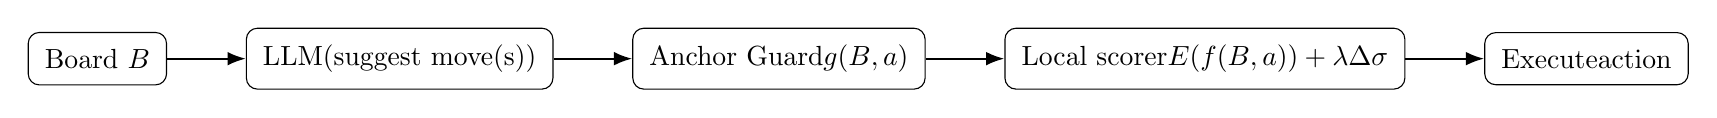
\begin{tikzpicture}[
  node distance=10mm,
  box/.style={draw, rounded corners, align=center, inner sep=6pt},
  arr/.style={-Latex, thick}
]
\node[box] (board) {Board $B$};
\node[box, right=of board] (llm) {LLM\newline (suggest move(s))};
\node[box, right=of llm] (guard) {Anchor Guard\newline $g(B,a)$};
\node[box, right=of guard] (rank) {Local scorer\newline $E(f(B,a)) + \lambda\Delta\sigma$};
\node[box, right=of rank] (exec) {Execute\newline action};

\draw[arr] (board) -- (llm);
\draw[arr] (llm) -- (guard);
\draw[arr] (guard) -- (rank);
\draw[arr] (rank) -- (exec);
\end{tikzpicture}
\caption{Hybrid pipeline: treat the LLM as a candidate generator; apply deterministic safety and local scoring before executing an action.}
\label{fig:pipeline}
\end{figure}

\begin{figure}[t]
\centering
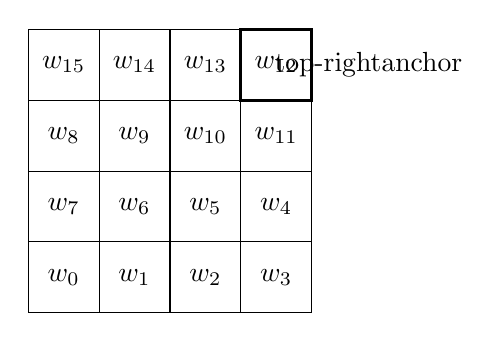
\begin{tikzpicture}[scale=0.9]
\foreach \r in {0,...,3} {
  \foreach \c in {0,...,3} {
    \draw (\c, -\r) rectangle (\c+1, -\r-1);
  }
}
\node at (0.5, -0.5) {$w_{15}$};
\node at (1.5, -0.5) {$w_{14}$};
\node at (2.5, -0.5) {$w_{13}$};
\node at (3.5, -0.5) {$w_{12}$};
\node at (0.5, -1.5) {$w_{8}$};
\node at (1.5, -1.5) {$w_{9}$};
\node at (2.5, -1.5) {$w_{10}$};
\node at (3.5, -1.5) {$w_{11}$};
\node at (0.5, -2.5) {$w_{7}$};
\node at (1.5, -2.5) {$w_{6}$};
\node at (2.5, -2.5) {$w_{5}$};
\node at (3.5, -2.5) {$w_{4}$};
\node at (0.5, -3.5) {$w_{0}$};
\node at (1.5, -3.5) {$w_{1}$};
\node at (2.5, -3.5) {$w_{2}$};
\node at (3.5, -3.5) {$w_{3}$};
\draw[very thick] (3, 0) rectangle (4, -1);
\node[align=center] at (4.8, -0.5) {top-right\newline anchor};
\end{tikzpicture}
\caption{Illustrative ``snake'' positional weighting: higher weights near the top-right anchor.}
\label{fig:snake}
\end{figure}

\section{Discussion}
Measured results show that the prompt-preference proxy does not reach 2048 in 200 games, while deterministic reranking improves average score yet still fails to reach 2048. In contrast, 4-ply expectimax achieves 49.0\% Win@2048, supporting the thesis that multi-step lookahead is critical. For true LLM controllers, the strongest practical direction is to combine (i) invariant-preserving constraints, (ii) local multi-step search or value estimation, and (iii) retrieval of situation-specific rules from logged play.

\section{Limitations}
The reported \texttt{llm\_\*} results come from offline proxy policies and do not measure real LLM latency, cost, or sampling variability. A full networked LLM evaluation should report decoding configuration, timeouts, caching, and rate limits.

\section{Conclusion}
We studied practical methods to improve LLM-style decision making in 2048. In a reproducible offline benchmark, deterministic reranking nearly doubled score but did not yield wins, while expectimax achieved 49.0\% Win@2048. These results indicate that reliable winning behavior requires multi-step planning and/or stronger value estimation, and that LLMs are most effective when used as strategic priors combined with deterministic constraints and local search.

\bibliographystyle{plain}
\begin{thebibliography}{9}
\bibitem{aima}
S. Russell and P. Norvig.
\newblock \emph{Artificial Intelligence: A Modern Approach}.
\newblock Pearson, 3rd edition, 2009.

\bibitem{mcts}
C. Browne, E. Powley, D. Whitehouse, et al.
\newblock A survey of Monte Carlo tree search methods.
\newblock \emph{IEEE Transactions on Computational Intelligence and AI in Games}, 4(1):1--43, 2012.
\end{thebibliography}

\end{document}
